\section{The Power Rule}
\label{sec:power}

This section is a very algebraic section and you should get lots of practice. When you tell someone you have studied calculus, this is the one skill they will expect you to have.

\subsection{Main Results}
These are the simplest rules -- rules for the basic functions. We won't prove each of these rules; we'll just use them. But first, let's look at a few examples so that we can see they make sense.

\begin{example}
Find the derivative of $f(x)=135.$

\begin{solution} Think about this one graphically. The graph of $f(x)$ is a horizontal line, so its slope is zero:
$$f'(x)=0 \enspace .$$
\end{solution}\end{example}
This obviously generalizes.
\begin{theorem}
The derivative of a constant is zero.

$$\dfrac{d}{dx}c = 0$$
\end{theorem}

\begin{example}
Find the derivative of $f(x)=5x+2$.

\begin{solution} This is a linear function, so its graph is its own tangent line! The slope of the tangent line, the derivative, is the slope of the line:
$$f'(x)=5$$
\end{solution}\end{example}

\begin{theorem}
The derivative of a linear function is its slope.

$$\dfrac{d}{dx}(mx+b) = m$$
\end{theorem}

\begin{example}
Find the derivative of $f(x)=x^2$.

\begin{solution} Recall the formal definition of the derivative:
$$f'(x)=\lim_{h\to 0} \dfrac{f(x+h)-f(x)}{h} \enspace .$$
Using our function $f(x)=x^2$, we use the distributive property to show that $f(x+h)=(x+h)^2=x^2+2xh+h^2$. Then
\begin{align*}
			f'(x) &= \lim_{h\to 0} \dfrac{f(x+h)-f(x)}{h}\\
			 &= \lim_{h\to 0} \dfrac{x^2+2xh+h^2-x^2}{h}\\
			 &= \lim_{h\to 0} \dfrac{2xh+h^2}{h}\\
			 &= \lim_{h\to 0} \dfrac{h(2x+h)}{h}\\
			 &= \lim_{h\to 0} (2x+h)\\
			 &= 2x \enspace .
		\end{align*}
From all that, we find that $f'(x)=2x$.
\end{solution}\end{example}

Luckily, there is a handy rule we use to skip using the limit for all power functions.

\begin{theorem}[Power Rule\index{Power rule}\index{Derivative rules!Power rule}]
\label{thm:powerrule}
For all real $n$, we have
$$\dfrac{d}{dx}x^n = nx^{n-1} \enspace .$$
\end{theorem}

\subsection{Polynomials and Power Functions}

Combining Theorem \ref{thm:powerrule} with the Sum and Difference Rule (Theorem \ref{thm:sumdiffderiv}) and the Constant Multiple Rule (Theorem \ref{thm:constmultderiv}, we can easily find the derivative of any polynomial. 

\begin{example}
Find the derivative of $g(x)=4x^3$.

\begin{solution} Using the Power Rule, we know that if $f(x)=x^3$, then $f'(x)=3x^2$. Notice that $g(x)$ is 4 times the function $f(x)$. So we have:
$$g'(x) = \dfrac{d}{dx}4x^3 = 4\dfrac{d}{dx}x^3 = 4\cdot 3x^2=12x^2 \enspace .$$
\end{solution}\end{example}

\begin{example}
Find the derivative of $p(x)=17x^{10}+13x^8-1.8x+1003$.

\begin{solution} 
    \begin{align*}
		\dfrac{d}{dx}\left( 17x^{10}+13x^8-1.8x+1003 \right) &= \dfrac{d}{dx}\left( 17x^{10} \right)+\dfrac{d}{dx}\left( 13x^8 \right)-\dfrac{d}{dx}\left( 1.8x \right)+\dfrac{d}{dx}\left( 1003 \right)\\
		 &= 17\dfrac{d}{dx}\left( x^{10} \right)+13\dfrac{d}{dx}\left( x^8 \right)-1.8\dfrac{d}{dx}\left( x \right)+\dfrac{d}{dx}\left( 1003 \right)\\
		 &= 17\left(10x^9\right)+13\left(8x^7\right)-1.8\left(1\right)+0\\
		 &= 170x^9+104x^7-1.8
	\end{align*}
\end{solution}\end{example}

You don't have to show every single step. Do be careful when you're first working with the rules, but pretty soon you'll be able to just write down the derivative directly:

\begin{example}
Find $\dfrac{d}{dx}(17x^2-33x+12).$

\begin{solution} Writing out the rules, we'd write
$$\dfrac{d}{dx}(17x^2-33x+12)=17(2x)-33(1)+0=34x-33 \enspace.$$

Once you're familiar with the rules, you can, in your head, multiply the 2 times the 17 and the 33 times 1, and just write
$$\dfrac{d}{dx}(17x^2-33x+12)=34x-33 \enspace .$$
\end{solution}\end{example}

The Power Rule works even if the power is negative or a fraction. In order to apply it, first translate all roots and basic rational expressions using exponents.

\begin{example}
Find the derivative of $y=3\sqrt{t}-\dfrac{4}{t^4}$.

\begin{solution} The first step is to rewrite the functions using exponents:  
    $$y=3\sqrt{t}-\dfrac{4}{t^4} = 3t^{1/2}-4t^{-4} \enspace .$$
Now you can take the derivative.
	\begin{align*}
    	y' = \dfrac{d}{dt}\left( 3t^{1/2}-4t^{-4} \right) &= 3\left(\dfrac{1}{2}t^{-1/2}\right)-4\left(-4t^{-5}\right) \\
		&= \dfrac{3}{2}t^{-1/2}+16t^{-5} \enspace . 
		\end{align*}
If there is a reason to, you can rewrite the derivative using radicals and positive exponents: 
$$y'= \dfrac{3}{2}t^{-1/2}+16t^{-5} = \dfrac{3}{2\sqrt{t}}+\dfrac{16}{t^5}$$
\end{solution}\end{example}

Be careful when finding the derivatives with negative exponents.

We can immediately apply these rules to solve the problem we started the chapter with -- finding a tangent line.

\begin{example}
Find the equation of the line tangent to $g(t)=10-t^2$ when $t=2$.

\begin{solution} The slope of the tangent line is the value of the derivative. We can compute $g'(t)=-2t$. To find the slope of the tangent line when $t=2$, evaluate the derivative at that point. The slope of the tangent line is $g'(2) = -2\cdot 2 = -4$.

To find the equation of the tangent line, we also need a point on the tangent line. Since the tangent line touches the original function at $t=2$, we can find the point by evaluating the original function: $g(2)=10-2^2 = 10-4 =6$. The tangent line must pass through the point $(2, 6)$.

Using the point-slope equation of a line, the tangent line will have equation $y-6=-4(t-2)$. Simplifying to slope-intercept form, the equation is $y=-4t+14$.

Graphing $y=g(t)$ and $y=-4t+14$, we can verify this line is indeed tangent to the curve.

\begin{figure}[!ht]
  \centering
    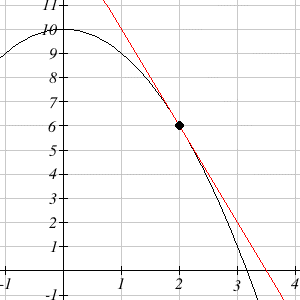
\includegraphics[width=0.4\textwidth]{img/chap2/image036.png}
    %\caption{$y=g(x)$}
    %\label{fig:2-2-gx}
\end{figure}
\end{solution}\end{example}

We can also use these rules to help us find the derivatives we need to interpret the behavior of a function.

\begin{example}
In a memory experiment, a researcher asks the subject to memorize as many words from a list as possible in 10 seconds. Recall is tested, then the subject is given 10 more seconds to study, and so on. Suppose the number of words remembered after $t$ seconds of studying could be modeled by $W(t)=4t^{2/5}$. Find and interpret $W'(20)$.

\begin{solution} $W'(t)=4 \cdot \dfrac{2}{5}t^{-3/5} \dfrac{\mbox{ words}}{\mbox{ second}} =\dfrac{8}{5}t^{-3/5}\dfrac{\mbox{ words}}{\mbox{ second}}$, so $W'(20)=\dfrac{8}{5}\cdot 20^{-3/5}\dfrac{\mbox{ words}}{\mbox{ second}}\approx   0.2652$ words per second.

Since $W(t)$ is measured in words and $t$ is in seconds, $W'$ has units ``words per second.'' $W'(20)\approx 0.2652$ words per second means that after 20 seconds of studying, the subject is learning about 0.27 more words for each additional second of studying.
\end{solution}\end{example}

\begin{example}
  \label{ex:2-7-11}
The cost to produce $x$ items is $C(x) = \sqrt{x}$ hundred dollars.
    \begin{enumerate}[label=(\alph*)]
    \item What is the cost to produce 100 items? 101 items? What is cost of the 101st item?

    \begin{solution}
     The cost to produce 100 items is $C(100)=\sqrt{100}$ hundred dollars $= \$1000$ and $C(101)=\$1004.99$, so it costs $\$4.99$ for that 101st item. By the definition of marginal cost\index{Cost!marginal}\index{Marginal cost}, the marginal cost is $\$4.99$.
    \end{solution}
    \item Calculate $C'(x)$ and evaluate $C'(100)$. How does $C'(100)$ compare with the last answer in Part (a)?
    
    \begin{solution} 
    Let's rewrite $C(x) = \sqrt{x} = x^{1/2}$ hundred dollars, the cost for $x$ items. $C'(x)= \dfrac{1}{2}x^{-1/2}$ hundred dollars per item, so $C'(100)=\dfrac{1}{2\sqrt{100}} = \dfrac{1}{20}$ hundred dollars per item $= \$5.00$ per item.
Note how close these answers are! This shows (again) why it's OK that we use both definitions for marginal cost.
    \end{solution}
    \end{enumerate}
\end{example}

\begin{example}
The demand\index{Demand}, $D$, for a product at a price of $p$ dollars is given by $D(p)=200-0.2p^2$. Find the marginal revenue\index{Marginal revenue} when the price is \$10.

\begin{solution} First we need to form a revenue\index{Revenue} equation. Since revenue is price times quantity, $R(p) = p\cdot D(p)$, and the demand equation shows the quantity of product that can be sold at price $p$. So we have:
$$R(p)=\left(p\, \frac{\mbox{dollars}}{\mbox{item}}\right) \cdot (D(p) \mbox{ items}) = p\cdot (200-0.2p^2) \mbox{ dollars} = 200p-0.2p^3 \enspace \mbox{dollars}.$$
Now we can find marginal revenue by finding the derivative:
$$R'(p)=200\cdot 1 - 0.2\cdot 3p^2 = 200-0.6p^2 \enspace \mbox{dollars per dollar}.$$
At a price of $\$10$, $R'(10)=200-0.6\cdot 10^2 = 200-0.6\cdot 100 = 200 - 60 = \$140$ per dollar.

Notice the units for $R'(p)$ are dollars (of revenue) per dollar (of price), so $R'(10)=140$ means that if the price per item is \$10, then the revenue would increase by \$140 for each dollar that the price per item is increased.
\end{solution}\end{example}

\subsection{Exercises}

